\documentclass{beamer}

\usepackage[utf8]{inputenc}
\usepackage{default}
\usepackage{graphicx}
\usepackage{float}
\usepackage{url}
\usepackage{hyperref}
\usepackage{menukeys}

\usepackage{tikz, times}
\usetikzlibrary{mindmap,backgrounds}
\pagestyle{empty}


%Python stuff:
%--------------------------------------------------------------------
% Default fixed font does not support bold face
\DeclareFixedFont{\ttb}{T1}{txtt}{bx}{n}{6} % for bold
\DeclareFixedFont{\ttm}{T1}{txtt}{m}{n}{6}  % for normal

% Custom colors
\usepackage{color}
\definecolor{deepblue}{rgb}{0,0,0.5}
\definecolor{deepred}{rgb}{0.6,0,0}
\definecolor{deepgreen}{rgb}{0,0.5,0}

\usepackage{listings}

% Python style for highlighting
\newcommand\pythonstyle{\lstset{
language=Python,
basicstyle=\ttm,
otherkeywords={self},             % Add keywords here
keywordstyle=\ttb\color{deepblue},
emph={MyClass,__init__},          % Custom highlighting
emphstyle=\ttb\color{deepred},    % Custom highlighting style
stringstyle=\color{deepgreen},
frame=tb,                         % Any extra options here
showstringspaces=false            % 
}}


% Python environment
\lstnewenvironment{python}[1][]
{
\pythonstyle
\lstset{#1}
}
{}

% Python for external files
\newcommand\pythonexternal[2][]{{
\pythonstyle
\lstinputlisting[#1]{#2}}}

% Python for inline
\newcommand\pythoninline[1]{{\pythonstyle\lstinline!#1!}}
%--------------------------------------------------------------------



\begin{document}

\section*{Outline}
\begin{frame}
 \tableofcontents
\end{frame}

\section{Introduction}
\begin{frame}
 \frametitle{Analysator}
 \begin{figure}
  \centering
  \includegraphics[width=\textwidth]{../images/analysator.jpg}
  \label{fig:mayavi_example}
 \end{figure}
\end{frame}

\begin{frame}
 \frametitle{What is Analysator}
 \begin{enumerate}
  \item An analysis tool developed for vlasiator
  \item Originally developed as an array reader for vlsv files
  \item Another aim: \emph{pointn'click tool} to get a velocity distributions
  \item Functions optimized with Scipy and Numpy libraries (close to C performance)
 \end{enumerate}
\end{frame}

\begin{frame}
 \frametitle{Functions}
 \begin{enumerate}
  \item Reading and writing \emph{numpy} arrays with \emph{VLSV} files
  \item Various \emph{analysis} tools
  \begin{enumerate}
   \item time-evolution of cells
   \item cut-throughs
   \item pitch angle distributions
   \item Accessing velocity distributions
   \item ..
  \end{enumerate}
  \item Plotting Vlasiator \emph{grids} using MayaVi library
  \item An interface to Urs' superb \emph{particle pusher}
  \item Full easy-to-use \emph{documentation} for every function
  \item Can be combined with \emph{every} python module and function
 \end{enumerate}
\end{frame}

\begin{frame}[fragile]
 \frametitle{Example}
 \begin{python}[basicstyle=\tiny]
  # We are interested in reading data from the cell whose ID is 75
 
  import pytools as pt # Import Analysator
  
  # Open a vlsv file for reading
  vlsvReader = pt.vlsvfile.VlsvReader('bulk.0003710.vlsv')
  
  # Read a variable at cell id 75
  rho = vlsvReader.read_variable( name='rho', cellids=75 )
 \end{python}
\end{frame}

\begin{frame}
 \frametitle{Important notes}
 Documentation can be found at \url{https://github.com/fmihpc/analysator/wiki}
\end{frame}


\section{Concepts}

\begin{frame}
 \frametitle{Modules in Analysator}
 \begin{center}
 \scalebox{0.5} {
  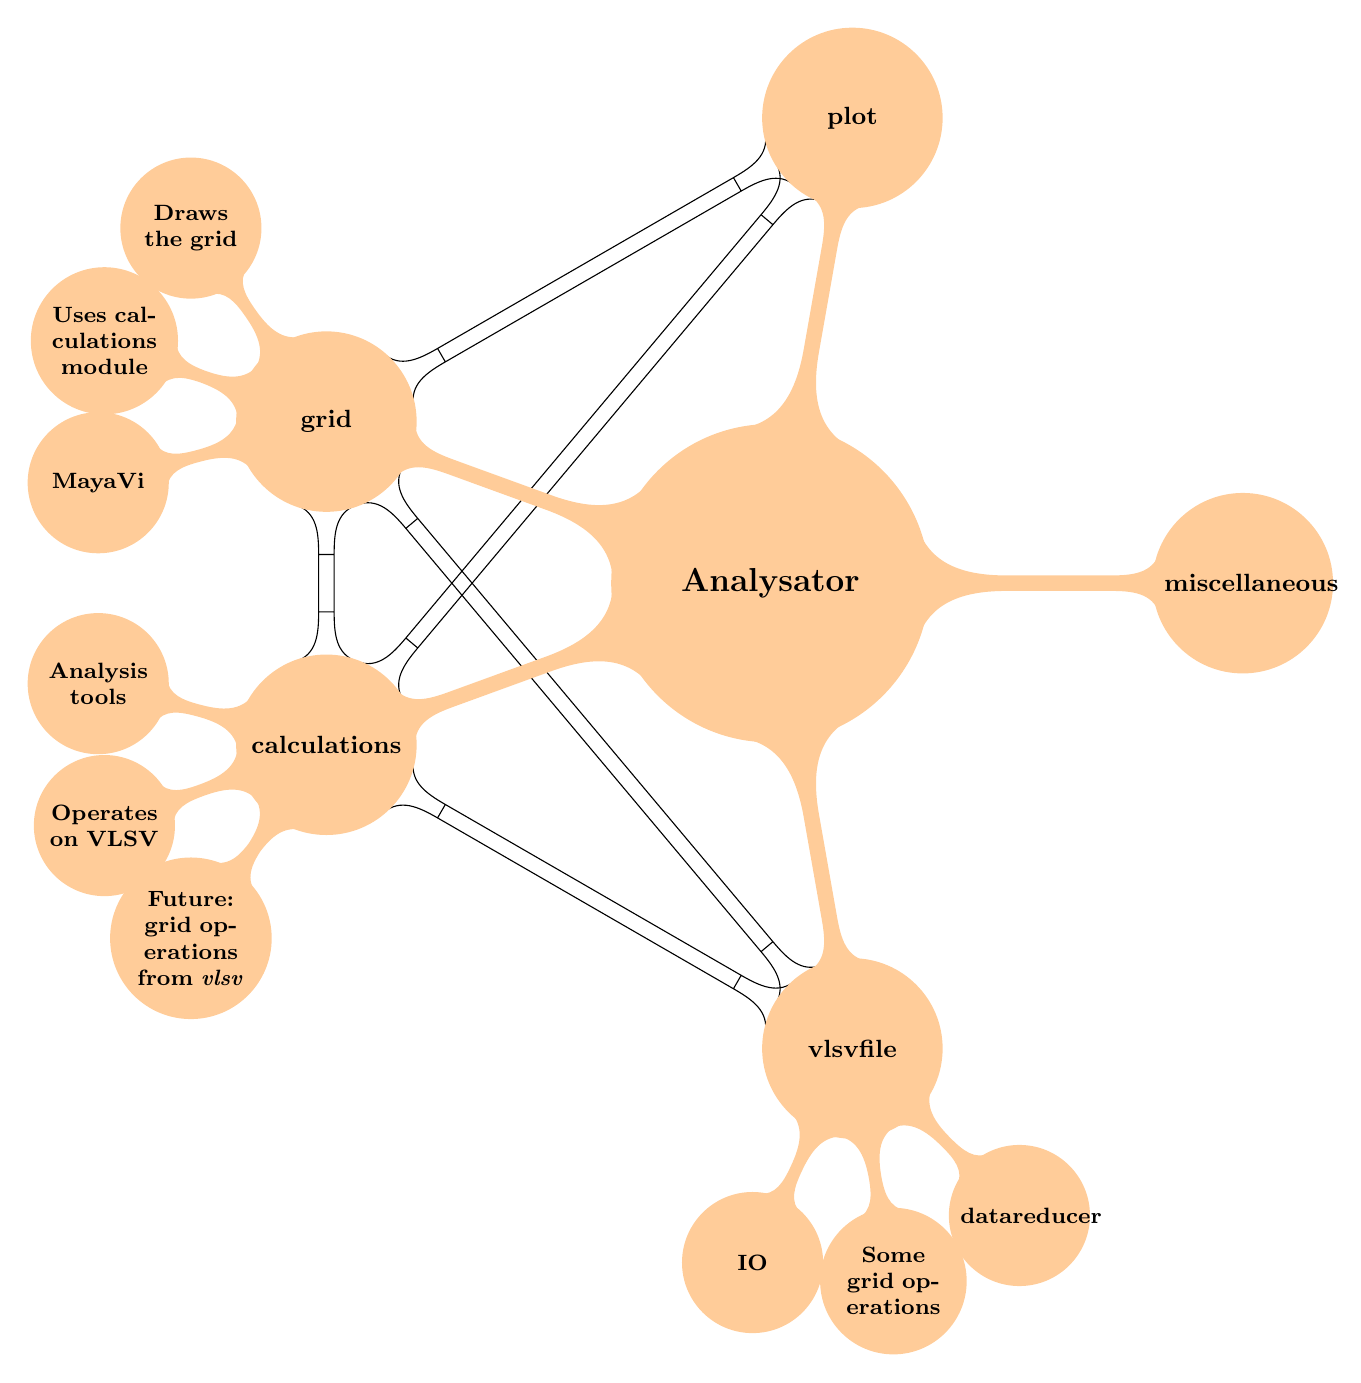
\begin{tikzpicture}[mindmap, grow cyclic, every node/.style=concept, concept color=orange!40, 
     level 1/.append style={level distance=6cm,sibling angle=80},
     level 2/.append style={level distance=3cm,sibling angle=35},] 


   \node{\textbf{Analysator}}
     child{ node[concept](calc) {\textbf{calculations}} child{node{\textbf{Analysis tools}}} child{node{\textbf{Operates on VLSV}}} child{node{\textbf{Future: grid operations from \emph{vlsv}}}} }
     child{ node[concept](vlsv){\textbf{vlsvfile}} child{node{\textbf{IO}}} child{node{\textbf{Some grid operations}}} child{node{\textbf{datareducer}}} }
     child{ node[concept](misc){\textbf{miscellaneous}} }
     child{ node[concept](plot){\textbf{plot}} }
     child{ node[concept](grid){\textbf{grid}} child{node{\textbf{Draws the grid}}} child{node{\textbf{Uses calculations module}}} child{node{\textbf{MayaVi}}} };
     
   \begin{pgfonlayer}{background}
    \draw [circle connection bar]
    (vlsv) edge (calc) edge (grid)
    (calc) edge (grid) edge (plot)
    (grid) edge (plot);
   \end{pgfonlayer}
  \end{tikzpicture}
 }
 \end{center}
\end{frame}

\begin{frame}[fragile]
 \frametitle{Navigation}
 
 \emph{Navigating} through the code important
 
 \begin{python}[basicstyle=\tiny]
  # Import analysator
  import pytools as pt
  
  vlsvReader = pt.vlsvfile.VlsvReader('test.vlsv') #What?
  
  cut_through = pt.calculations.cut_through(vlsvReader, point1=[0,0,0], point2=[2,5e6,0])
 \end{python}
 
 \begin{enumerate}
  \item Otherwise you need to remember
  \begin{enumerate}
   \item The name of the cut\_through function
   \item The first function argument: \emph{vlsvReader}
   \item The second argument: \emph{point1}
   \item The third argument: \emph{point2}
   \item The second and third argument's format and dimensions \emph{(3d list)}
  \end{enumerate}
 \end{enumerate}

\end{frame}



\begin{frame}[fragile]
 \frametitle{Navigation (the \emph{most} important part)}
 \begin{python}[basicstyle=\tiny]
  # Import analysator
  import pytools as pt
  
  pt.
 \end{python}
 \keys{tab}
 \begin{python}[basicstyle=\tiny]
In [2]: pt.
pt.calculations    pt.grid            pt.plot            
pt.filemanagement  pt.miscellaneous   pt.vlsvfile    
 \end{python}
\end{frame}

\begin{frame}[fragile]
 \frametitle{Navigation (the \emph{most} important part)}
 \begin{python}[basicstyle=\tiny]
  # Import analysator
  import pytools as pt
  
  pt.calculations.
 \end{python}
 \keys{tab}
 \begin{python}[basicstyle=\tiny]
pt.calculations.cell_time_evolution
pt.calculations.cut3d
pt.calculations.cut_through
pt.calculations.fit
pt.calculations.fourier
pt.calculations.gyrophase_angles_from_file
pt.calculations.lineout
pt.calculations.pitch_angles
pt.calculations.VariableInfo
 \end{python}
\end{frame}

\begin{frame}[fragile]
 \frametitle{Navigation (the \emph{most} important part)}
 \begin{python}[basicstyle=\tiny]
  # Import analysator
  import pytools as pt
  
  pt.calculations.cut_through?
 \end{python}
 \keys{Enter}
 \begin{python}[basicstyle=\tiny]
In [2]: pt.calculations.cut_through?
Definition: pt.calculations.cut_through(vlsvReader, point1, point2)
Docstring:
Returns cell ids and distances from point 1 for every cell in a line between 
given point1 and point2

:param vlsvReader:       Some open VlsvReader
:type vlsvReader:        :class:`vlsvfile.VlsvReader`
:param point1:           The starting point of a cut-through line
:param point2:           The ending point of a cut-through line
:returns: an array containing cell ids, coordinates and distances in the following 
format: [cell ids, distances, coordinates]

.. code-block:: python

   Example:
   vlsvReader = VlsvReader("testfile.vlsv")
   cut_through = cut_through(vlsvReader, [0,0,0], [2,5e6,0])
   cellids = cut_through[0]
   distances = cut_through[1]
   print "Cell ids: " + str(cellids)
   print "Distance from point 1 for every cell: " + str(distances)

 \end{python}
\end{frame}

\begin{frame}[fragile]
 \frametitle{Navigation summary}
 \begin{python}[basicstyle=\tiny]
  pt.calculations.
 \end{python}
 \keys{tab} Autocompletion
 \begin{python}[basicstyle=\tiny]
  pt.calculations?
 \end{python}
 \keys{Enter} Getting documentation
\end{frame}


\section{Basics}

\begin{frame}
 \frametitle{Basic usage}
 \begin{enumerate}
  \item Open a \emph{vlsv} file
  \item Read from the \emph{vlsv} file
  \item Operate on the data
 \end{enumerate}
\end{frame}

\begin{frame}[fragile]
 \frametitle{Basic usage}
 \begin{python}[basicstyle=\tiny]
  # Import analysator
  import pytools as pt
  
  # Open a vlsv file
  vlsvReader = pt.vlsvfile.VlsvReader('test.vlsv')
  
  # Read vlsv data
  rho = vlsvReader.read_variable('rho')
  
 \end{python}

\end{frame}


\section{Hands-on}

\begin{frame}[fragile]
 
 \frametitle{Hands-on}
 \begin{center}
  \textbf{Hands-on}
 \end{center}
 
 Summary of the basics:
 \begin{enumerate}
  \item Remember to \emph{import analysator}
  \item Nearly every script starts by opening a \emph{vlsv} file
  \item \keys{tab} to navigate
  \item ? + \keys{Enter} to get documentation
 \end{enumerate}
 
 Note: if you have virtualbox you have to set up a shared folder:
 \begin{verbatim}
  sudo mount -t vboxsf -o rw,uid=1000,gid=1000 \
  vlsv_data $HOME/share
 \end{verbatim}
 
 \scalebox{0.1} {
  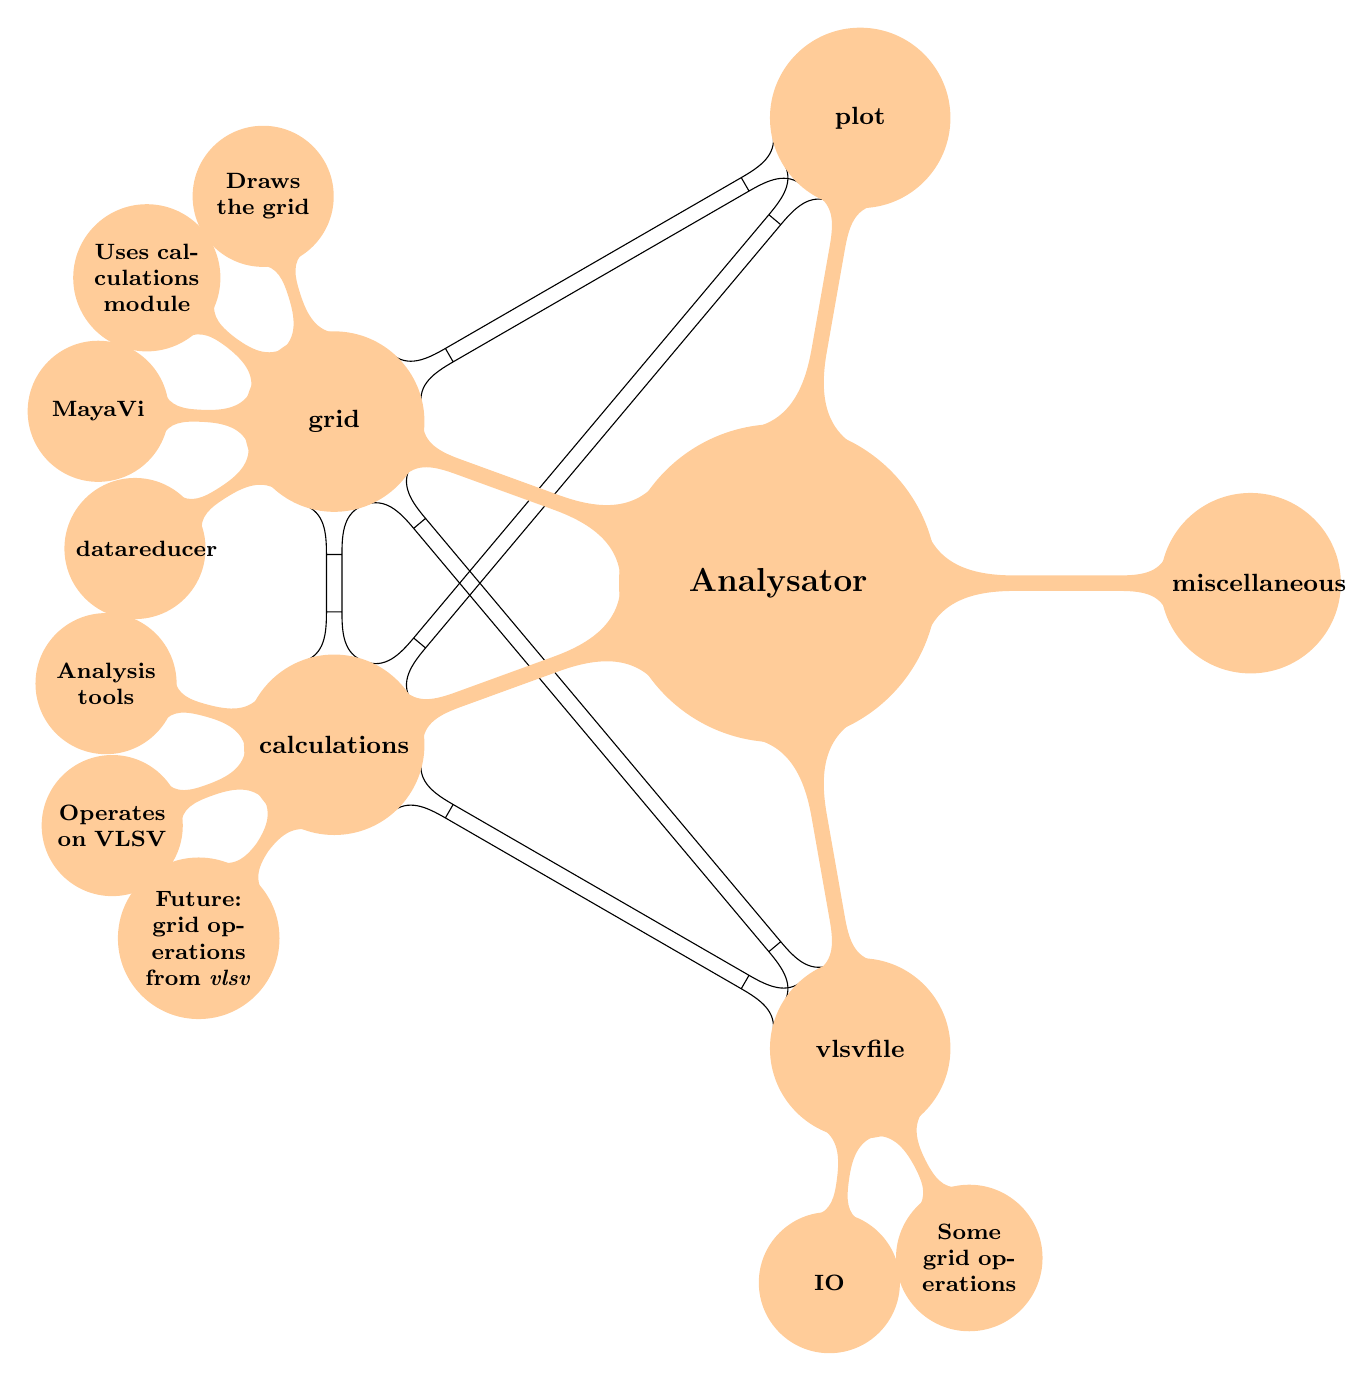
\begin{tikzpicture}[mindmap, grow cyclic, every node/.style=concept, concept color=orange!40, 
     level 1/.append style={level distance=6cm,sibling angle=80},
     level 2/.append style={level distance=3cm,sibling angle=35},] 


   \node{\textbf{Analysator}}
     child{ node[concept](calc) {\textbf{calculations}} child{node{\textbf{Analysis tools}}} child{node{\textbf{Operates on VLSV}}} child{node{\textbf{Future: grid operations from \emph{vlsv}}}} }
     child{ node[concept](vlsv){\textbf{vlsvfile}} child{node{\textbf{IO}}} child{node{\textbf{Some grid operations}}} }
     child{ node[concept](misc){\textbf{miscellaneous}} }
     child{ node[concept](plot){\textbf{plot}} }
     child{ node[concept](grid){\textbf{grid}} child{node{\textbf{Draws the grid}}} child{node{\textbf{Uses calculations module}}} child{node{\textbf{MayaVi}}} child{node{\textbf{datareducer}}} };
     
   \begin{pgfonlayer}{background}
    \draw [circle connection bar]
    (vlsv) edge (calc) edge (grid)
    (calc) edge (grid) edge (plot)
    (grid) edge (plot);
   \end{pgfonlayer}
  \end{tikzpicture}
 }
\end{frame}

\section{Plotting}

\begin{frame}
 \frametitle{Plotting}
 \begin{center}
 \scalebox{0.8} {
  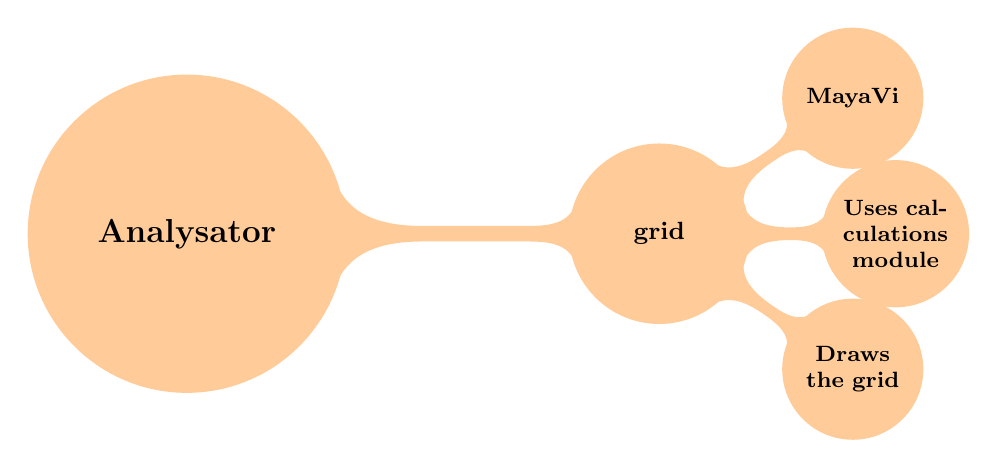
\begin{tikzpicture}[mindmap, grow cyclic, every node/.style=concept, concept color=orange!40, 
     level 1/.append style={level distance=6cm,sibling angle=80},
     level 2/.append style={level distance=3cm,sibling angle=35},] 


   \node{\textbf{Analysator}}
     child{ node[concept](grid){\textbf{grid}} child{node{\textbf{Draws the grid}}} child{node{\textbf{Uses calculations module}}} child{node{\textbf{MayaVi}}} };
  \end{tikzpicture}
 }
 \end{center}
\end{frame}

\begin{frame}
 \frametitle{Plotting}
 The most important concepts
 \begin{enumerate}
  \item How to plot
  \item How to use MayaVi
  \item How to use the Analysator's \emph{pointnclick} interface
 \end{enumerate}
\end{frame}

\begin{frame}[fragile]
 \frametitle{Plotting}
 \begin{center}
  \scalebox{0.5}{\vbox{ \begin{enumerate}
   \item How to plot
  \end{enumerate} } }
 \end{center}
 Plotting can be done simply by feeding a vlsv file to the grid class as follows:
 \begin{python}[basicstyle=\tiny]
  # Import Analysator
  import pytools as pt
  
  # Open a vlsv file
  vlsvReader = pt.vlsvfile.VlsvReader('test.vlsv')
  
  # Plot rho
  grid = pt.grid.MayaviGrid(vlsvReader, variable='rho')
 \end{python}
\end{frame}

\begin{frame}[fragile]
 \frametitle{Plotting}
 \begin{center}
  \scalebox{0.5}{\vbox{ \begin{enumerate}
   \item How to plot
   \item How to use MayaVi
  \end{enumerate} } }
 \end{center}
 \begin{figure}
  \centering
  \includegraphics[width=\textwidth]{../images/none.png}
  \caption{\tiny{Example plot with Mayavi, highlighting options and pointnclick tool.}}
  \label{fig:mayavi_example}
 \end{figure}
\end{frame}

\begin{frame}[fragile]
 \frametitle{Plotting}
 \begin{center}
  \scalebox{0.5}{\vbox{ \begin{enumerate}
   \item How to plot
   \item How to use MayaVi
 \end{enumerate} } }
 
 \begin{figure}
  \centering
  \includegraphics[height=0.2\textheight]{../images/none.png}
  \caption{\tiny{Example plot with Mayavi, highlighting options and pointnclick tool.}}
  \label{fig:mayavi_example2}
 \end{figure}
 
 \begin{enumerate}
  \item \keys{Scroll} to zoom
  \item \keys{Mouse 3} to move the image
  \item \keys{Mouse 1} + \keys{Hold} to pan the image
  \item \keys{Mouse 1} to click
 \end{enumerate}

 \end{center}
 
\end{frame}

\begin{frame}[fragile]
 \frametitle{Plotting}
 \begin{center}
  \scalebox{0.5}{\vbox{ \begin{enumerate}
   \item How to plot
   \item How to use MayaVi
   \item How to use the Analysator's \emph{pointnclick} interface
  \end{enumerate} } }
 \end{center}
 \emph{Pointnclick} options:
 \begin{enumerate}
  \item None
  \item Velocity\_space\_nearest\_cellid
  \item Velocity\_space\_nearest\_cellid\_iso\_surface
  \item Pitch\_angle
  \item Gyrophase\_angle (Made by \emph{Yann}, yay)
  \item Cut\_through
 \end{enumerate}

 Click \keys{Mouse 1} somewhere on the \emph{grid}
\end{frame}

\begin{frame}[fragile]
 \frametitle{Plotting}
 \begin{center}
  \scalebox{0.5}{\vbox{ \begin{enumerate}
   \item How to plot
   \item How to use MayaVi
   \item How to use the Analysator's \emph{pointnclick} interface
  \end{enumerate} } }
 \end{center}
 
 \tiny{Sorry about the horribly small text..}
 
 \begin{figure}
  \centering
  \includegraphics[width=\textwidth]{../images/velocity_space_nearest_cellid_iso_surface.png}
  \label{fig:mayavi_example3}
 \end{figure}
\end{frame}

\section{Hands-on}

\begin{frame}[fragile]
 \frametitle{Hands-on}
 
 To get started:
 
 \begin{python}[basicstyle=\tiny]
  grid = pt.grid.MayaviGrid(vlsvReader, 'rho')
 \end{python}
 
 Summary:
 
 \begin{enumerate}
  \item \keys{Mouse scroll} to zoom
  \item \keys{Mouse 3} to move the image
  \item \keys{Mouse 1} + \keys{Hold} to pan
  \item \keys{Mouse 1} to use the Analysator \emph{pointnclick}
 \end{enumerate}

 
 \tiny{Note on \emph{pointnclick} \textbf{cut-through option}:
 
 Press \keys{Mouse 1} in two places, and there is a \emph{field} where you have to type:}
 \begin{verbatim}
  plot rho
 \end{verbatim}
\end{frame}


\begin{frame}[fragile]
 \scalebox{0.1} {
  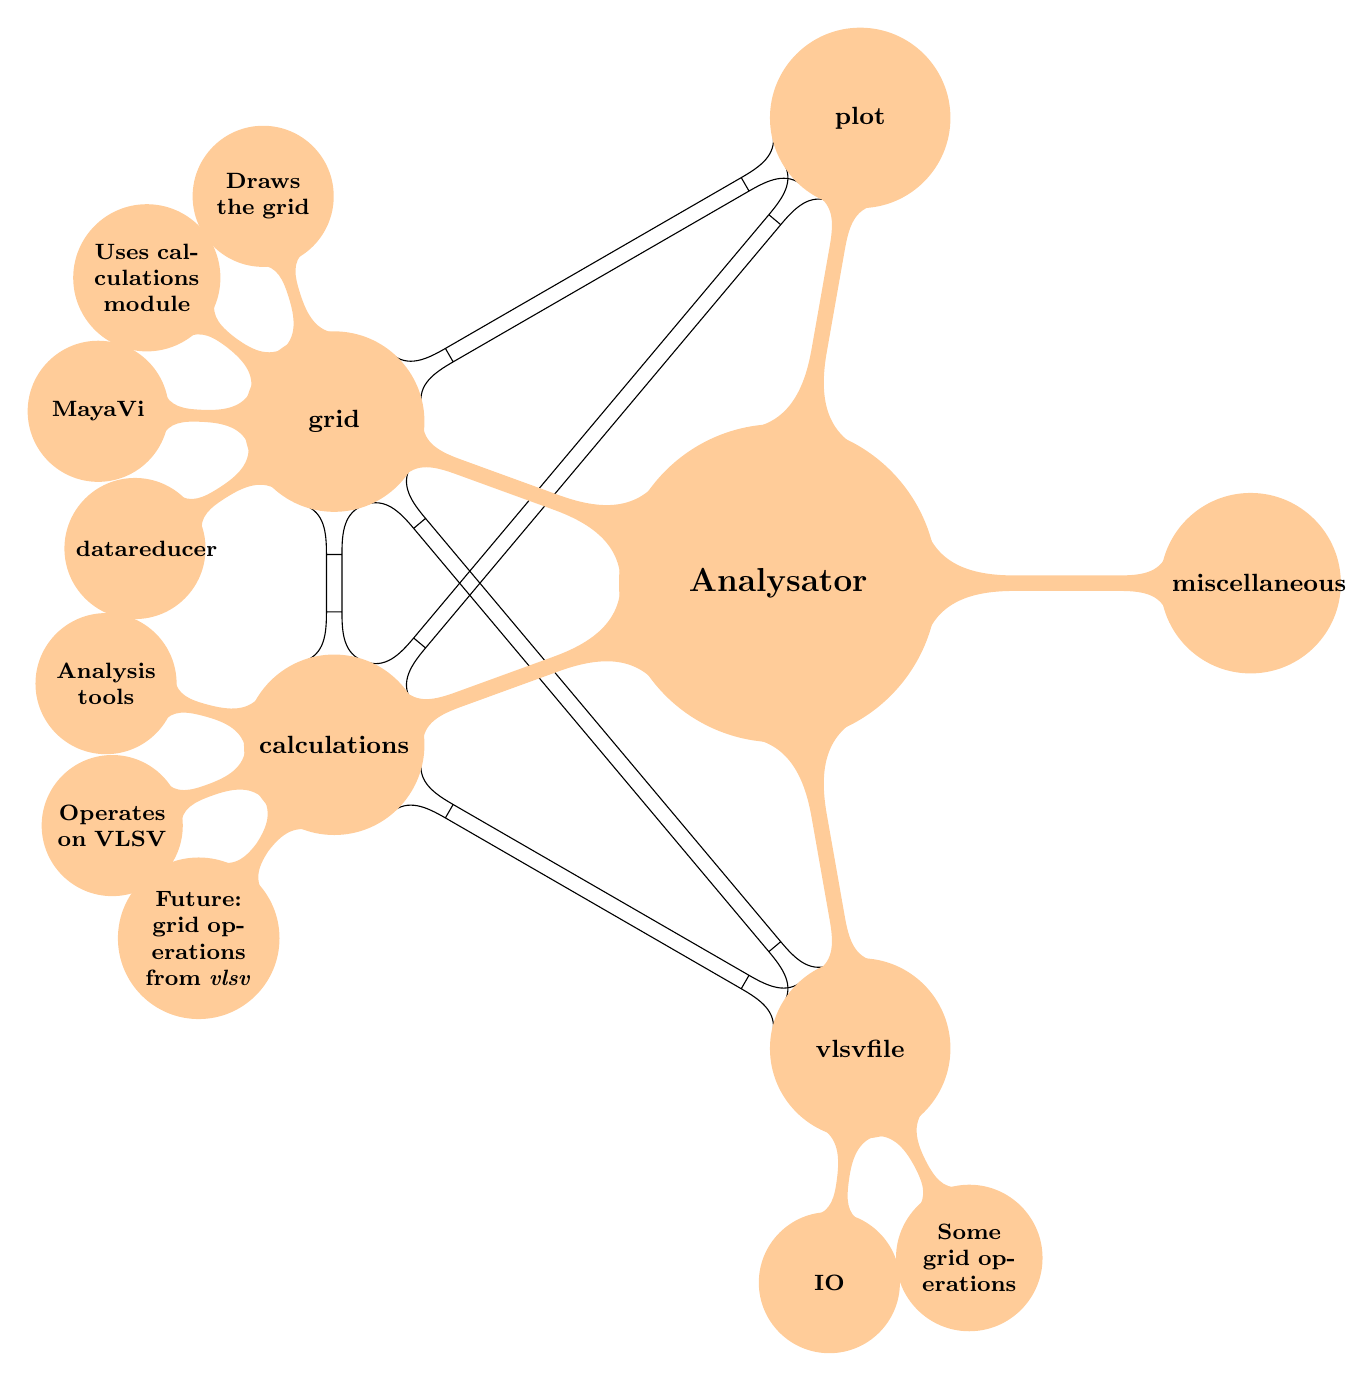
\begin{tikzpicture}[mindmap, grow cyclic, every node/.style=concept, concept color=orange!40, 
     level 1/.append style={level distance=6cm,sibling angle=80},
     level 2/.append style={level distance=3cm,sibling angle=35},] 


   \node{\textbf{Analysator}}
     child{ node[concept](calc) {\textbf{calculations}} child{node{\textbf{Analysis tools}}} child{node{\textbf{Operates on VLSV}}} child{node{\textbf{Future: grid operations from \emph{vlsv}}}} }
     child{ node[concept](vlsv){\textbf{vlsvfile}} child{node{\textbf{IO}}} child{node{\textbf{Some grid operations}}} }
     child{ node[concept](misc){\textbf{miscellaneous}} }
     child{ node[concept](plot){\textbf{plot}} }
     child{ node[concept](grid){\textbf{grid}} child{node{\textbf{Draws the grid}}} child{node{\textbf{Uses calculations module}}} child{node{\textbf{MayaVi}}} child{node{\textbf{datareducer}}} };
     
   \begin{pgfonlayer}{background}
    \draw [circle connection bar]
    (vlsv) edge (calc) edge (grid)
    (calc) edge (grid) edge (plot)
    (grid) edge (plot);
   \end{pgfonlayer}
  \end{tikzpicture}
 }
 \frametitle{Example from \emph{calculations}}
 \begin{python}[basicstyle=\tiny]
  # Import analysator
  import pytools as pt
  
  # Open a vlsv file
  vlsvReader = pt.vlsvfile.vlsvReader('testfile.vlsv')
  
  # Get a cut-through starting at (x=0, y=0; z=0) to (x=2, y=5e6, z=0) :
  cut_through = pt.calculations.cut_through(vlsvReader, point1=[0,0,0], point2=[2,5e6,0])
  
  # We now have the cut_through, so now we want to print cellids:
  cellids = cut_through[0]
  print cellids
 \end{python}

\end{frame}




\end{document}
